\documentclass[12pt,a4paper]{article}

% Packages
\usepackage{amsmath, amssymb}
\usepackage{graphicx}
\usepackage{siunitx} 
\usepackage{caption}
\usepackage{geometry}
\usepackage{url}
\usepackage{cite}
\usepackage{hyperref}
\usepackage{listings}
\usepackage{listings-rust}
\usepackage{xurl}
\usepackage{siunitx}

\lstset{language=Rust, style=boxed}
\geometry{margin=1in}
\graphicspath{{/images}}

\title{Sensors and Actuators for Robotics and
Automation\\Term Project Progress Report III}
\author{Kanisorn Sangchai (ID: 6538020621)}
\date{October 20, 2025}

\begin{document}

\maketitle

\section{Introduction}
This report documents the implementation of Analog-to-Digital Conversion, software configuration, and sensor value read for a thermistor-based temperature sensor system. The STM32H743VIT6 core board by WeAct Studio is used to perform the analog to digital conversion and transmit the measured sensor values via UART communication. The source code for this project can be found in this GitHub repository: \url{https://github.com/Kanisorn-S/sara-project}. The source code for Milestone 2 can be found in the \texttt{Milestone-3} branch: \url{https://github.com/Kanisorn-S/sara-project/tree/Milestone-3}.

\begin{figure}[h]
    \centering
    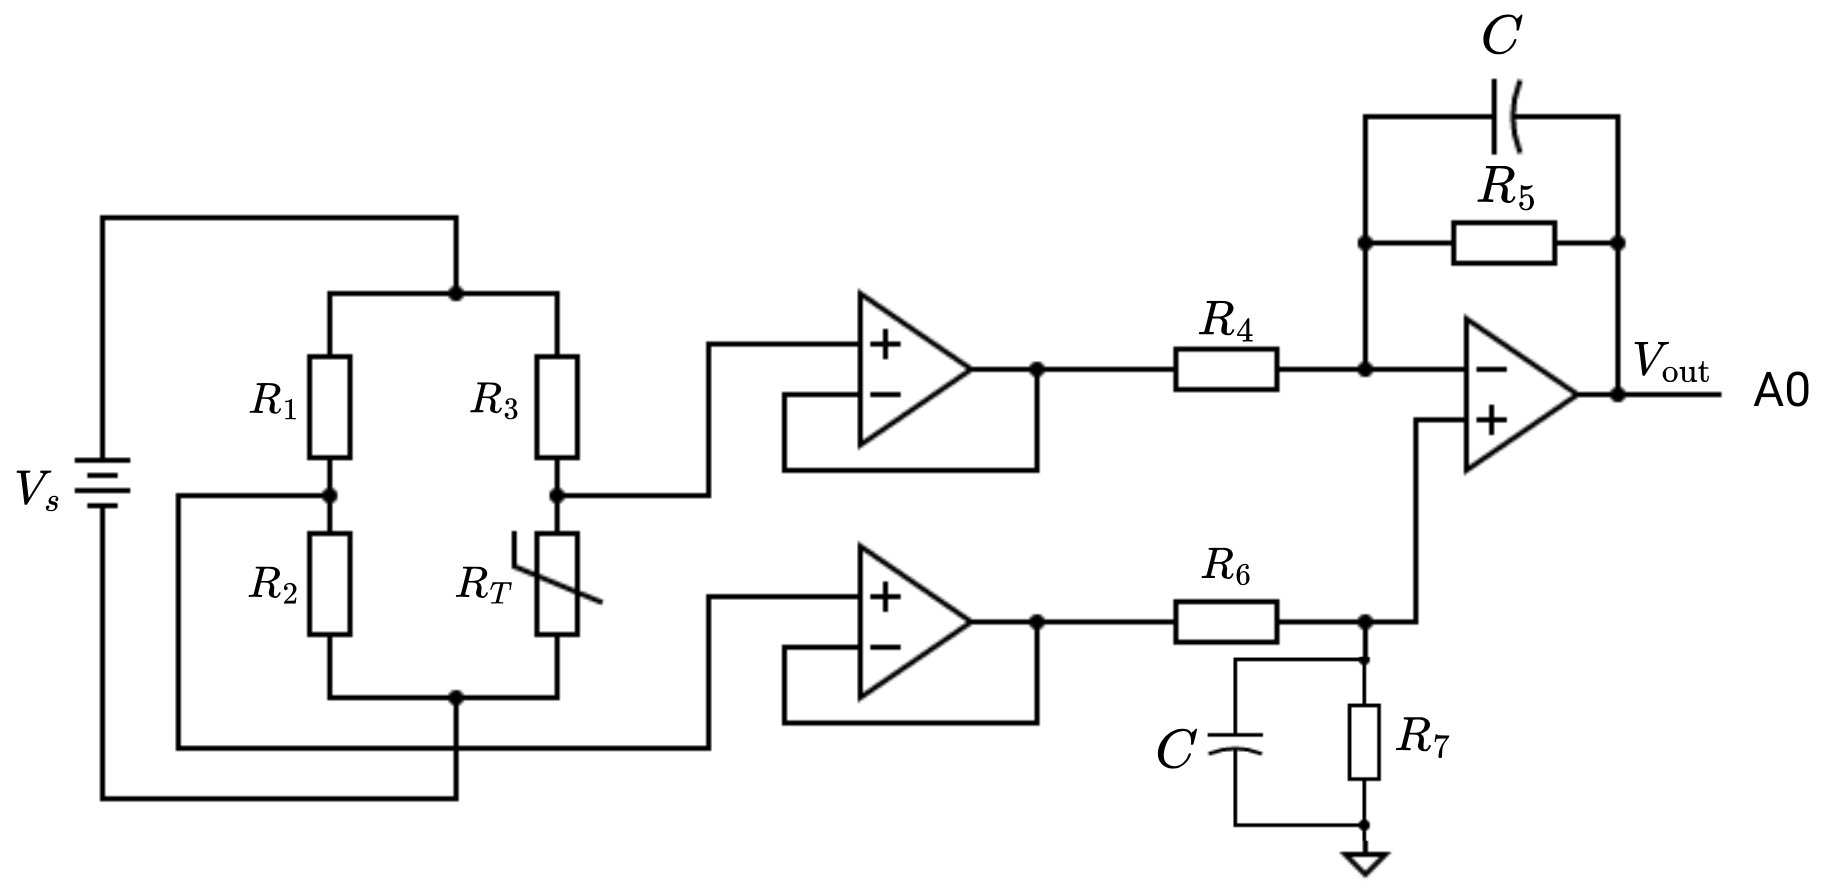
\includegraphics[width=0.9\textwidth]{images/circuit_diagram.png}
    \caption{Original circuit diagram with an adjustable voltage divider added to control the temperature}
    \label{fig:circuit}
\end{figure}

\section{Circuit Design}
An adjustable voltage divider was added to the original circuit design, as shown in Figure~\ref{fig:circuit}, to manipulate the temperature of the thermistor.

The voltage divider consists of 
\begin{itemize}
    \item Potentiometer
    \item Fixed Resistor
\end{itemize} 
By adjusting the potentiometer, the voltage across the fixed resistor can be changed, which in turn changes its temperature.

\subsection{Components}
\subsubsection{Potentiometer}
For this project, a B Linear Taper 1 Turn Rotary Potentiometer is used to adjust the voltage divider ratio, thus adjusting the voltage across the fixed resistor. The voltage across the fixed resistor $V_{\text{Heat}}$ can be calculated using the formula:

\begin{equation*}
    V_{\text{Heat}} = V_s \cdot \frac{R_{\text{Fixed}}}{R_{\text{Fixed}} + R_{\text{Pot}}}
\end{equation*}

Where:

\begin{equation*}
    R_{\text{Pot}} = R_{\text{Pot, Max}} \cdot \frac{\theta}{\theta_{\text{Max}}}
\end{equation*}

Giving us:

\begin{equation}
    \label{eq:v-heat-theta}
    V_{\text{Heat}} = V_s \cdot \frac{R_{\text{Fixed}}}{R_{\text{Fixed}} + R_{\text{Pot, Max}} \cdot \frac{\theta}{\theta_{\text{Max}}}}
\end{equation}

The selected potentiometer is the WH148 B Linear Taper 1 Turn Rotary Potentiometer with a maximum resistance of $\SI{10}{k\ohm}\pm 20\%$~\cite{potentiometer}.

\subsubsection{Fixed Resistor}
For this project, a fixed resistor is used in conjunction with the potentiometer to form the voltage divider. The value of the fixed resistor $R_{\text{Heat}}$ is chosen to be $\SI{560}{\ohm}\pm 1\%$. This value is selected to ensure that the voltage across the fixed resistor can be adjusted within a suitable range for heating purposes.

\section{Mathematical Model}

\subsection{Temperature Manipulation}
We use our STM32H743VIT6 Core Board's \SI{3.3}{\volt} to power the adjustable voltage divider, giving us $V_s=\SI{3.3}{\volt}$. To manipulate the temperature of the thermistor, we can adjust the angle $\theta$ of the potentiometer. From Equation~\ref{eq:v-heat-theta}, we can see that the maximum voltage across the fixed resistor occurs when $\theta = \SI{0}{\degree}$, which gives us:
\begin{equation*}
    V_{\text{Heat, Min}} = V_s \cdot \frac{R_{\text{Fixed}}}{R_{\text{Fixed}} + 0} = V_s = \SI{3.3}{\volt}
\end{equation*}
While the minimum voltage occurs when $\theta = \theta_{\text{Max}}$, which gives us:
\begin{equation*}
    V_{\text{Heat, Max}} = V_s \cdot \frac{R_{\text{Fixed}}}{R_{\text{Fixed}} + R_{\text{Pot, Max}}} = \SI{3.3}{\volt} \cdot \frac{\SI{560}{\ohm}}{\SI{560}{\ohm} + \SI{10}{k\ohm}} = \SI{0.175}{\volt}
\end{equation*}
Calculating for the error,
\begin{align*}
    \frac{\delta V_{\text{Heat}}}{V_{\text{Heat}}} &=  \frac{\delta R_\text{fixed}}{R_\text{fixed}} + \frac{\delta (R_\text{fixed} + R_\text{pot})}{R_\text{fixed} + R_\text{pot}} \\
    &= 0.01 + \frac{0.01 \cdot R_\text{fixed} + 0.2 \cdot R_\text{pot}}{R_\text{fixed} + R_\text{pot}} \\
    &= 0.01 + \frac{0.01 \cdot 560 + 0.2 \cdot 10000}{560 + 10000} \\
    &\approx 0.01 + 0.19 \\
    &\approx 0.2
\end{align*}

\begin{table}[h!]
\centering
\begin{tabular}{lccc}
\hline
\textbf{DIN size} & \textbf{0204} & \textbf{0207} & \textbf{0414} \\
\hline
Thermal time constant, $\tau_w$ (s) & 2 & 5 & 20 \\
Thermal resistance, $R_{th}$ (K/W)  & 400 & 250 & 170 \\
\hline
\end{tabular}
\caption{Examples of resistor thermal time constant and thermal resistance on leaded cylindrical components. (from~\cite{thermal-resistance})}
\label{tab:thermal-resistance}
\end{table}

To find the change in temperature of the fixed resistor based on the voltage across it, we first need to find the resistor's thermal resistance $R_{\text{th}}$. Our resistor's body length is $\SI{10}{mm}$, the closest DIN standard size to our resistor's body length is 0414~\cite[pp.~13]{din}. From Table~\ref{tab:thermal-resistance}, we can find that the thermal resistance for a 0414 resistor is $R_{\text{th}} = \SI{170}{K/W}$. The temperature change $\Delta T$ of the fixed resistor can be calculated using the formula:
\begin{equation*}
    \Delta T = R_{\text{th}} \cdot P
\end{equation*}
Where $P$ is the power dissipated by the resistor, which can be calculated using the formula:
\begin{equation*}
    P = \frac{V_{\text{Heat}}^2}{R_{\text{Heat}}}
\end{equation*}
Combining the two equations, we get:
\begin{equation}
    \Delta T = R_{\text{th}} \cdot \frac{V_{\text{Heat}}^2}{R_{\text{Heat}}}
    \label{eq:delta-t}
\end{equation}
To get the full equation, we combine Equation~\ref{eq:v-heat-theta} and Equation~\ref{eq:delta-t} to get:
\begin{equation}
    \Delta T = R_{\text{th}} \cdot \frac{\left(V_s \cdot \frac{R_{\text{Fixed}}}{R_{\text{Fixed}} + R_{\text{Pot, Max}} \cdot \frac{\theta}{\theta_{\text{Max}}}}\right)^2}{R_{\text{Heat}}}
    \label{eq:full-delta-t}
\end{equation}


\label{sec:math-model}


\section{Demonstration and Verification}

\section{Conclusion}


\newpage
\bibliographystyle{IEEEtran}
\bibliography{ref}

\end{document}
